 \documentclass[12pt]{article}

\usepackage{epsfig}
\usepackage{comment}
\usepackage{natbib}
\usepackage{natbibmnfix}
\usepackage{graphicx}
\usepackage{color}
\usepackage{subfig}
\usepackage{bmpsize}
\usepackage{caption}
\usepackage{amsmath}
\usepackage{breqn}
\usepackage{wrapfig}
\usepackage{lipsum}
\usepackage{float}
%\usepackage{newcaptions} % changes the appearance of captions
\usepackage{url}
\usepackage{soul} % enables a better version of "\underline{}", called '\ul{}", which for instance permits linebreaks

\setul{1.5pt}{.4pt}
\newcommand{\UL}[1]{\ul{#1}}


\newcounter{dummy}
\def\@biblabel#1{\hspace*{\labelsep}[#1]}

\newcommand{\df}{\delta_{\rm F}}
\newcommand\atf{ATF}
\newcommand\scott[1]{\textcolor{blue}{\textbf{[Scott:}~#1} ]}

\def\lya{Ly$\alpha$}
\def\lyb{Ly$\beta$}
\def\etal{{\rm et~al.\ }}
\def\hmpc{\;h^{-1}{\rm Mpc}}
\def\hgpc{\;h^{-1}{\rm Gpc}}
\def\hkpc{h^{-1}{\rm kpc}}
\def\kpc{{\rm kpc}}
\def\kms{{\rm \;km\;s^{-1}}}
\def\shear{\langle \gamma^{2} (\theta) \rangle}
\newcommand{\phiv}{\mbox{\boldmath$\phi$}}
\newcommand{\thetav}{\mbox{\boldmath$\theta$}}
\def\pef{\par\noindent\hangindent 15pt}
\def\simlt{\lower.5ex\hbox{$\; \buildrel < \over \sim \;$}}
\def\lesssim{\lower.5ex\hbox{$\; \buildrel < \over \sim \;$}}
\def\simgt{\lower.5ex\hbox{$\; \buildrel > \over \sim \;$}}
\def\apj{{\it Astrophys. J.}}
\def\jcap{{\it  J. Cosmo. \& Astroparticle Phys.}}
\def\aj{{\it Astron. J.}}
\def\mnras{{\it Mon. Not. R. astr. Soc.}}
\newcommand{\apjl}{ApJL}
\newcommand{\nat}{Nature}
\newcommand{\araa}{ARA\&A}
\newcommand{\apjs}{ApJS}
\newcommand{\aap}{A\&A}
\newcommand{\pasp}{PASP}
\newcommand{\sfig}[2]{
\begin{center}
\includegraphics[width=#2]{#1}
\end{center}
        }
\newcommand{\Sjpg}[2]{
    \begin{figure}[htb]
    \sfig{./#1.jpg}{.9\columnwidth}
    \caption{{\small #2}}
    \label{fig:#1}
    \end{figure}
}
\newcommand{\Sfig}[2]{
    \begin{figure}[htb]
    \sfig{./#1.pdf}{.9\columnwidth}
    \caption{{\small #2}}
    \label{fig:#1}
    \end{figure}
}
\newcommand{\Spng}[2]{
    \begin{figure}[htb]
    \sfig{#1.png}{.9\columnwidth}
    \caption{{\small #2}}
    \label{fig:#1}
    \end{figure}
}

\newcommand{\Sfigtwo}[3]{
        \begin{figure}[htbp]
\sfig{#1.eps}{.3\columnwidth}
\sfig{#2.eps}{.3\columnwidth}
\caption{{\small #3}}
\label{fig:#1}
\end{figure}
}
\newcommand\be{\begin{equation}}
\newcommand{\Rf}[1]{\ref{fig:#1}}
\newcommand{\rf}[1]{\ref{fig:#1}}
\def\ee{\end{equation}}
\def\bea{\begin{eqnarray}}
\def\eea{\end{eqnarray}}
\newcommand{\vs}{\nonumber\\}
\newcommand{\ec}[1]{Eq.~(\ref{eq:#1})}
\newcommand{\Ec}[1]{(\ref{eq:#1})}
\newcommand{\eql}[1]{\label{eq:#1}}
\newcommand\cov{{\rm Cov}}
\newcommand\cl{{\mathcal{C}_l}}
\usepackage[margin=3.0cm]{geometry}
\usepackage{pslatex}
\newcommand\fnl{f_{\rm NL}}
\newcommand{\wh}[1]{\textcolor{blue}{[#1]}}
\newcommand{\tred}[1]{\textcolor{red}{[#1]}}

\newcommand\cp{C^{pri}}
\newcommand\ci{C^{ISW}}
\newcommand\cg{C^{gg}}
\newcommand\cgt{C^{g-ISW}}
\newcommand\tob{T^{\rm obs}}
\newcommand\aob{a^{\rm obs}}
\newcommand\tisw{T^{\rm ISW}}
\newcommand\aisw{a^{\rm ISW}}
\newcommand\si{C^{\rm ISW}_l}
\newcommand\sig[1]{C^{\rm g_{#1}-ISW}_l}
\newcommand\sg[2]{C^{\rm g_{#1}g_{#2}}_l}
\newcommand\tp{T^p}


%
% definitions
%
% A useful Journal macro
\def\Journal#1#2#3#4{{#1} {\bf #2}, #3 (#4)}
% Some useful journal names
\def\NCA{\em Nuovo Cimento\ }
\def\NPB{{\em Nucl. Phys.} B\ }
\def\PLB{{\em Phys. Lett.}  B\ }
\def\PRL{{\em Phys. Rev. Lett.\ }}
\def\PRD{{\em Phys. Rev.} D\ }
\def\prd{{\em Phys. Rev.} D\ }
\def\ZPC{{\em Z. Phys.} C\ }
\def\apj{{\em Ap. J.\ }}
\def\apjl{{\em Ap. J. Lett.\ }}
\def\la{\hbox{${_{\displaystyle<}\atop^{\displaystyle\sim}}$}}
\def\ga{\hbox{${_{\displaystyle>}\atop^{\displaystyle\sim}}$}}



\baselineskip=11pt
\def\msun{{\rm M_{\odot}}}

%\textheight=24.3cm
%\textwidth=16.8cm

\begin{document}
\topmargin=-2.105cm
\oddsidemargin=-0.1cm
\evensidemargin=0cm

\begin{center}
{\bf PSC Proposal\\}
Yingzhang Chen
\end{center}

\begin{small}


\section{Introduction and Scientific Background}
Galaxy–galaxy (g–g) lensing is a powerful probe of the relation between galaxies and dark matter (DM) haloes, but  its  theoretical  interpretation  requires  a  careful  modelling  of  various  contributions,  such  as  the  contributions from  central  and  satellite  galaxies.  For  this  purpose, we developed a new method using the components of lensing shear $\gamma_1$ and $\gamma_2$ instead of tangential shear to extract information from the g–g weak lensing signal by comparing it to high-resolution dissipationless simulations that resolve subhaloes. We find that this method can better constrain subhalo masses and thus enabling us to further investigate halo-galaxy connections.

From the NFW density profile, we can derive the convergence field
\begin{equation}
    \kappa(\bm{\theta})=\frac{\Sigma(D_l\bm{\theta})}{\Sigma_{cr}}
\end{equation}
where
\begin{equation}
    \Sigma(\bm{\xi}) = \int \mathrm{d}z \rho(\xi_1,\xi_2,z)
\end{equation}
is the surface density, $\bm{\xi}=(\xi_1,\xi_2)$ is the impact two-vector in the lens plane, $z$ is the perpendicular coordinate to the lens plane.

\begin{equation}
    \Sigma_{cr} = \frac{1}{4\pi G} \frac{D_s}{D_l D_{ls}}
\end{equation}

The deflection angle can be expressed in terms of convergence as 
\begin{equation}
    \bm{\alpha}(\bm{\theta}) = \frac{1}{\pi}\int \mathrm{d}^2 \bm{\theta}'\kappa(\bm{\theta})\frac{\bm{\theta} - \bm{\theta}'}{|\bm{\theta} - \bm{\theta}'|^2}
\end{equation}

and 2-dimensional deflection potential:
\begin{equation}
    \Psi(\bm{\theta})=\frac{1}{\pi}\int \mathrm{d}^2 \bm{\theta}'\kappa(\bm{\theta})\mathrm{ln}|\bm{\theta} - \bm{\theta}'|
\end{equation}

such that:
\begin{equation}
    \bm{\alpha}(\bm{\theta}) =\nabla \Psi(\bm{\theta})
\end{equation}

$\Psi(\bm{\theta})$ then satisfies the 2-dimensional Poisson equation:
\begin{equation}
    \kappa(\bm{\theta}) = \frac{1}{2}\nabla^2 \Psi(\bm{\theta})
\end{equation}
the lensing mapping Jacobian matrix is:
\begin{equation}
    \mathcal{\bm{A}}(\bm{\theta}) = \delta_{ij} - \frac{\partial^2\Psi(\bm{\theta})}{\partial\theta_i\partial\theta_j} = \begin{pmatrix}
1-\kappa -\gamma_1 & \gamma_2 \\
\gamma_2 & 1-\kappa +\gamma_1
\end{pmatrix}
\end{equation}

So 
\begin{align}
    \gamma_1 &= \frac{A_{11}-A_{22}}{2} \\
    \gamma_2 &= A_{12}
\end{align}


\section{Progress to Date and Motivation for Future Work}


\begin{figure*}
 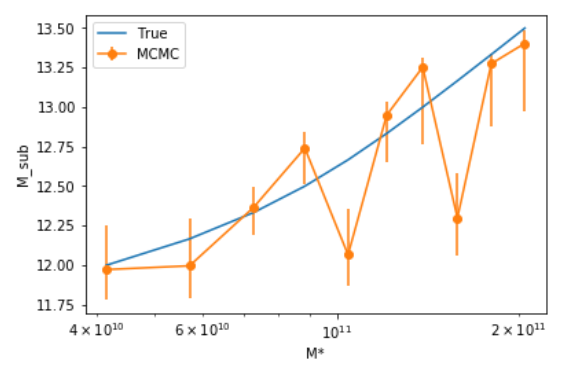
\includegraphics[width=\textwidth]{Fig1.png}
 \caption{This plot shows the MCMC result based on $\gamma_1$ and $\gamma_2$ method comparing with true value.
}
 \label{SM_HM_fig}
\end{figure*}




We constrain the subhalo masses using MCMC method, for a single sample case, the log-likelihood function is given by:
\begin{align*}
    \log \mathcal{L}(M \mid \mathcal{D}) &= \sum_k -\frac{1}{2}(\gamma^{theory}_{1,k}(M)-\gamma^{data}_{1,k})^T\Sigma^{-1}(\gamma^{theory}_{1,k}(M)-\gamma^{data}_{1,k}) \\ 
    & -\frac{1}{2} (\gamma^{theory}_{2,k}(M)-\gamma^{data}_{2,k})^T\Sigma^{-1}(\gamma^{theory}_{2,k}(M)-\gamma^{data}_{2,k}) 
\end{align*}

Where $\gamma^{theory}_{1,k}(M)$ and  $\gamma^{theory}_{2,k}(M)$ are the theoretic prediction of $\gamma_1$ and $\gamma_2$ at pixel $k$, the covariance matrix is assumed to be diagonal with:

\begin{align*}
    \Sigma &= diag(\sigma_{\gamma_{1}}^2, \sigma_{\gamma_{2}}^2,...,\sigma_{\gamma_{k}}^2)
\end{align*}

The total log-likelihood function is given by:
\begin{align*}
    \log \mathcal{L} = \sum_{i=1}^n p_i \sum_{j=1}^m  \log \mathcal{L}(M_{i}  \mid \mathcal{D}_{i,j})
\end{align*}

Where $n=10$ is the number of stellar mass bins, $m=50$ is the sampling number in each bin. $p_i$ is the lenses number factor:
\begin{align*}
    p_i = \frac{N_i}{m} \times \frac{S_{LSST}}{S_{cosmoDC2}}
\end{align*}

Where $N_i$ is the number of lenses in the $i$th mass bin between $z=0.3$ to $z=0.4$ in cosmoDC2 simulation, $S_{LSST}=20000 \mathrm{deg}^2$, $S_{cosmoDC2}=440 \mathrm{deg}^2$


\section{Proposed Computational Methods}

Given cosmological parameters in cosmoDC2, we first generate fake galaxies with subhalo masses and stellar masses. Then we fed the fake data to emcee, a module using affine invariant Markov chain Monte Carlo (MCMC) ensemble sampler (\url{https://github.com/dfm/emcee}). We ran a chain with 10 mass bins (10 parameters) with 10k steps.
%\newpage

\section{Computational Resources}
NERSC GPU

\end{small}
\bibliographystyle{plain}
\bibliography{refs}

\end{document}
